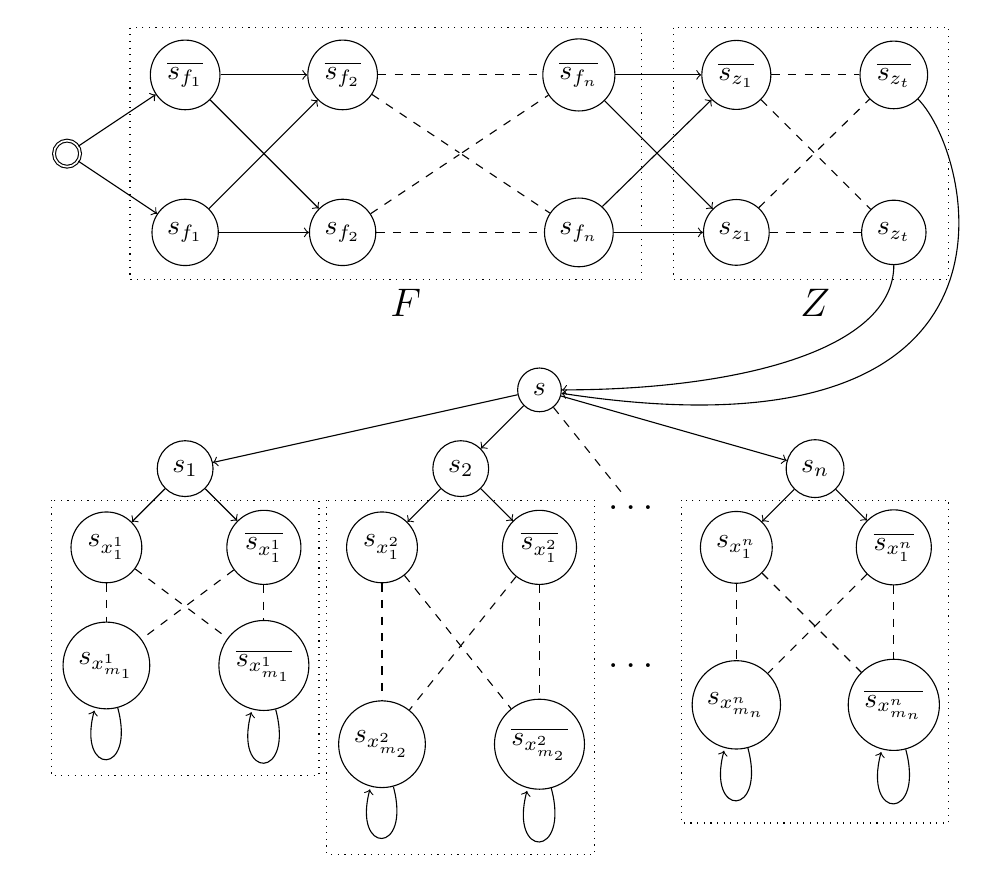
\begin{tikzpicture}

\path [use as bounding box] (-6.5,1.1) rectangle (5.5,-9.4);

\node [draw,double,circle] (v1) at (-6,-0.5) {$\sinit$};
\node [draw,circle] (v2) at (-4.5,-1.5) {$s_{f_1}$};
\node [draw,circle] (v3) at (-4.5,0.5) {$\overline{s_{f_1}}$};
\node [draw,circle] (v4) at (-2.5,-1.5) {$s_{f_2}$};
\node [draw,circle] (v5) at (-2.5,0.5) {$\overline{s_{f_2}}$};
\node [draw,circle] (v6) at (0.5,-1.5) {$s_{f_n}$};
\node [draw,circle] (v8) at (0.5,0.5) {$\overline{s_{f_n}}$};
\node [draw,circle] (v7) at (2.5,-1.5) {$s_{z_1}$};
\node [draw,circle] (v9) at (2.5,0.5) {$\overline{s_{z_1}}$};
\node [draw,circle] (v10) at (4.5,-1.5) {$s_{z_t}$};
\node [draw,circle] (v12) at (4.5,0.5) {$\overline{s_{z_t}}$};
\node [draw,circle] (v11) at (0,-3.5) {$s$};

\draw [->] (v1) edge (v2);
\draw [->] (v1) edge (v3);
\draw [->] (v2) edge (v4);
\draw [->] (v2) edge (v5);
\draw [->] (v3) edge (v4);
\draw [->] (v3) edge (v5);
\draw [->] (v6) edge (v7);
\draw [->] (v8) edge (v9);
\draw [->] (v6) edge (v9);
\draw [->] (v8) edge (v7);
\draw [dotted] (-5.2,1.1) rectangle (1.3,-2.1);
\draw [dotted] (1.7,1.1) rectangle (5.2,-2.1);


\node [inner sep=0, outer sep=0] (v15) at (-1,0.5) {};
\node [inner sep=0, outer sep=0] (v14) at (-1,-0.5) {};
\node [inner sep=0, outer sep=0] (v13) at (-1,-1.5) {};
\draw [dashed] (v4) edge (v13);
\draw [dashed] (v13) edge (v6);
\draw [dashed] (v4) edge (v14);
\draw [dashed] (v14) edge (v6);
\draw [dashed] (v5) edge (v14);
\draw [dashed] (v14) edge (v8);
\draw [dashed] (v5) edge (v15);
\draw [dashed] (v15) edge (v8);
\draw [dashed] (v7) edge (v10);
\draw [dashed] (v7) edge (v12);
\draw [dashed] (v9) edge (v10);
\draw [dashed] (v9) edge (v12);
\node at (3.5,-2.4) {\Large $Z$};
\node at (-1.7,-2.4) {\Large $F$};


\node [draw,circle] (v16) at (-4.5,-4.5) {$s_1$};
\node [draw,circle] (v17) at (-1,-4.5) {$s_2$};
\node [draw,circle] (v18) at (3.5,-4.5) {$s_n$};
\node [draw,circle] (v19) at (-5.5,-5.5) {$s_{x^1_1}$};
\node [draw,circle] (v20) at (-3.5,-5.5) {$\overline{s_{x^1_1}}$};
\node [draw,circle] (v21) at (-2,-5.5) {$s_{x^2_1}$};
\node [draw,circle] (v22) at (0,-5.5) {$\overline{s_{x^2_1}}$};
\node [draw,circle] (v23) at (2.5,-5.5) {$s_{x^n_1}$};
\node [draw,circle] (v24) at (4.5,-5.5) {$\overline{s_{x^n_1}}$};
\node [draw,circle] (v25) at (-5.5,-7) {$s_{x^1_{m_1}}$};
\node [draw,circle] (v26) at (-3.5,-7) {$\overline{s_{x^1_{m_1}}}$};
\node [draw,circle] (v27) at (-2,-8) {$s_{x^2_{m_2}}$};
\node [draw,circle] (v28) at (0,-8) {$\overline{s_{x^2_{m_2}}}$};
\node [draw,circle] (v29) at (2.5,-7.5) {$s_{x^n_{m_n}}$};
\node [draw,circle] (v30) at (4.5,-7.5) {$\overline{s_{x^n_{m_n}}}$};
\draw [->] (v11) edge (v16);
\draw [->] (v11) edge (v17);
\draw [->] (v11) edge (v18);
\node (v31) at (1.2,-5) {\Large \dots};
\node at (1.2,-7) {\Large \dots};
\draw [->] (v16) edge (v19);
\draw [->] (v16) edge (v20);
\draw [->] (v17) edge (v21);
\draw [->] (v17) edge (v22);
\draw [->] (v18) edge (v23);
\draw [->] (v18) edge (v24);
\draw [->] (v25) edge[loop below] (v25);
\draw [->] (v26) edge[loop below] (v26);
\draw [->] (v27) edge[loop below] (v27);
\draw [->] (v28) edge[loop below] (v28);
\draw [->] (v29) edge[loop below] (v29);
\draw [->] (v30) edge[loop below] (v30);
\draw [dashed] (v19) edge (v25);
\draw [dashed] (v19) edge (v26);
\draw [dashed] (v20) edge (v25);
\draw [dashed] (v20) edge (v26);
\draw [dashed] (v21) edge (v27);
\draw [dashed] (v21) edge (v28);
\draw [dashed] (v22) edge (v27);
\draw [dashed] (v22) edge (v28);
\draw [dashed] (v23) edge (v29);
\draw [dashed] (v23) edge (v30);
\draw [dashed] (v24) edge (v29);
\draw [dashed] (v24) edge (v30);
\draw [dashed] (v11) edge (v31);
\draw [dotted] (-6.2,-4.9) rectangle (-2.8,-8.4);
\draw [dotted] (-2.7,-4.9) rectangle (0.7,-9.4);
\draw [dotted] (1.8,-4.9) rectangle (5.2,-9);

\draw [->](v12) .. controls (5.5,-0.5) and (6.5,-4.5) .. (v11);
\draw [->](v10) .. controls (4.5,-3) and (2.5,-3.5) .. (v11);
\end{tikzpicture}